\section{Templates}




\subsection{Boat}
The boat template as the name infers is a model of the real boat. 
The boat is capable of carrying at most two persons and most have at least one adult to handle the boat. 
From the initial state, called still, the only possible edge is to the one person location. 
In this edge the boat listens for a handshake on the adultOn channel. 
When a person responds to the handskake the persons sailing time is transmitted through the global variable temp_sailtime. 
A function set_sailtime is used to set the sailtime to the lowest value, so the fastest person on the boats sailing time is the one used. 
temp_sailtime is reset to reduce the state space.
7 From the One person location there are three edges. 
Two edges to the two person loaction where eihter a child or an adult embarks. 
The adultOn edge is similar to the first edge described. 
The childOn edge does not need to synchronize a sailtime since the children does not control the boat. 
From both two person and the one person location an edge to the sailing locatoin is possible. 
Here a card calls the function verify, which is described in \ref{}. 
The sailing location has an invariant that makes sure it stays in the location for atleast the time it takes for the person to sail across. 
The only possible edge from the sailing location is to arrieved. 
This edge has a gaurd to make sure that the boat arrieves when it has stayed in sailing in a period equivalent to the sail_time. 
The edge broadcasts on allDisembark and makes all persons on the boat disembark. 
The local variable boatL is fliped to note that the boat has changed site. 
After the disembarkment the sail time is reset to the maximum sailtime and the postion of the people is verifyed. 
\begin{figure}%
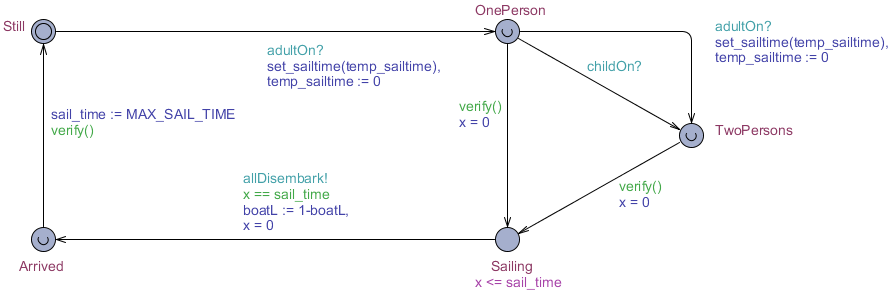
\includegraphics[width=\columnwidth]{pictures/boat.png}%
\caption{}%
\label{}%
\end{figure}
















\section{Person}
\begin{figure}%
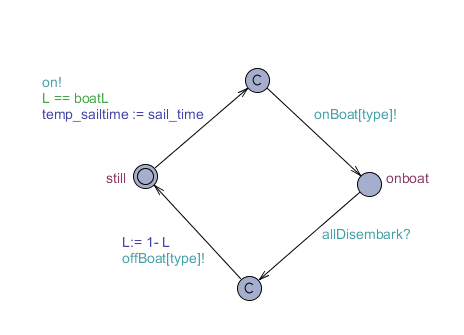
\includegraphics[width=\columnwidth]{pictures/person.png}%
\caption{}%
\label{}%
\end{figure}



















\section{Observer}
\begin{figure}%
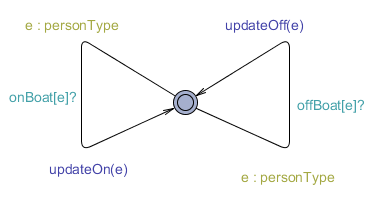
\includegraphics[width=\columnwidth]{pictures/observer.png}%
\caption{}%
\label{}%
\end{figure}




























\section{Observer}